\documentclass[12pt]{article} % размер шрифта

\usepackage{etex} % боремся с tex capacity exceeded
\usepackage{tikz} % картинки в tikz
\usepackage{microtype} % свешивание пунктуации

\usepackage{array} % для столбцов фиксированной ширины

\usepackage{indentfirst} % отступ в первом параграфе

\usepackage{sectsty} % для центрирования названий частей
\allsectionsfont{\centering} % приказываем центрировать все sections

\usepackage{amsmath} % куча стандартных математических плюшек
\usepackage{amssymb} % куча стандартных математических плюшек

\usepackage[top=1.5cm, left=1.3cm, right=1.3cm, bottom=1.5cm]{geometry} % размер текста на странице

\usepackage{lastpage} % чтобы узнать номер последней страницы

\usepackage{enumitem} % дополнительные плюшки для списков
%  например \begin{enumerate}[resume] позволяет продолжить нумерацию в новом списке
\usepackage{caption} % подписи к картинкам без плавающего окружения figure


\usepackage{fancyhdr} % весёлые колонтитулы
\pagestyle{fancy}
\lhead{Введение в теорию групп}
\chead{}
\rhead{КЛШ-42}
\lfoot{}
\cfoot{}
\rfoot{\thepage/\pageref{LastPage}}
\renewcommand{\headrulewidth}{0.4pt}
\renewcommand{\footrulewidth}{0.4pt}

\usepackage{url} % для вставки гиперссылок

\usepackage{todonotes} % для вставки в документ заметок о том, что осталось сделать
% \todo{Здесь надо коэффициенты исправить}
% \missingfigure{Здесь будет картина Последний день Помпеи}
% команда \listoftodos — печатает все поставленные \todo'шки

\usepackage{booktabs} % красивые таблицы
% заповеди из документации:
% 1. Не используйвертикальные линии
% 2. Не используйдвойные линии
% 3. Единицы измерения помещайв шапку таблицы
% 4. Не сокращай.1 вместо 0.1
% 5. Повторяющееся значение повторяйте, а не говори"то же"

\usepackage{fontspec} % поддержка разных шрифтов
\usepackage{polyglossia} % поддержка разных языков

\setmainlanguage{russian}
\setotherlanguages{english}

\setmainfont{Linux Libertine O} % выбираем шрифт
% можно также попробовать Helvetica, Arial, Cambria и т.Д.

% чтобы использовать шрифт Linux Libertine на личном компе,
% его надо предварительно скачать по ссылке
% http://www.linuxlibertine.org/index.php?id=91&L=1

\newfontfamily{\cyrillicfonttt}{Linux Libertine O}
% пояснение зачем нужно шаманство с \newfontfamily
% http://tex.stackexchange.com/questions/91507/

\AddEnumerateCounter{\asbuk}{\russian@alph}{щ} % для списков с русскими буквами
\setlist[enumerate, 2]{label=\asbuk*),ref=\asbuk*} % списки уровня 2 будут буквами а) б) ...

%% эконометрические и вероятностные сокращения
\DeclareMathOperator{\Cov}{Cov}
\DeclareMathOperator{\Corr}{Corr}
\DeclareMathOperator{\Var}{Var}
\DeclareMathOperator{\E}{E}
\def \hb{\hat{\beta}}
\def \hs{\hat{\sigma}}
\def \htheta{\hat{\theta}}
\def \s{\sigma}
\def \hy{\hat{y}}
\def \hY{\hat{Y}}
\def \v1{\vec{1}}
\def \e{\varepsilon}
\def \he{\hat{\e}}
\def \z{z}
\def \hVar{\widehat{\Var}}
\def \hCorr{\widehat{\Corr}}
\def \hCov{\widehat{\Cov}}
\def \cN{\mathcal{N}}

\def \ZZ{\mathbb{Z}}


\begin{document}

\section{Анонс курса}

Введение в теорию групп

Что общего между выворачиванием носков наизнанку, попытками повесить картину на два гвоздя, целыми числами, кубиком Рубика и вращениями геометрических фигур? Теория групп — это абстрактный язык, объединяющий эти и многие другие непохожие предметы и действия с ними.
Теория групп возникает повсюду: от поиска корней уравнений до описания симметрий кристаллов и атомов. А мы начнём с составления таблицы умножения для носков и перчаток :)

Требование к участникам: уметь делить с остатком.

Готов к численности: ~10-20 человек.


\section{Советы семинаристам (Артём Абанов)}
\begin{itemize}\itemsep 0.2\baselineskip
\item Начинать семинар с трёпа (2-3 минуты).
\item Не решать задачи у доски!
\item Школьников надо рассадить так, чтобы к любому можно было быстро подойти.
\item Каждый школьник делает задачи индивидуально. Для этого к семинарскому занятию надо быть готовым. Идеально иметь кучу задач написанных на карточках или отдельных клочках бумаги.
\item Ваша задача — подбирать каждому школьнику задачи чуть-чуть выше того уровня на котором ему/ей удобно и комфортно.
\item Когда школьник решил задачу — i) похвалить, ii) проверить размерность, iii) проверить/обратить внимание на предельные случаи: можно ли ответ понять без вычислений?
\item Если задача у школьника вызывает затруднение — похвалить и помочь коротким советом индивидуально.
\item Если затруднения продолжаются — похвалить, придумать подзадачу которая ему/ей по силам и сделать поправку на будущее.
\item Если замечаете, что школьники устали рассказать коротко какую-нибудь байку, лучше в тему.
\item Обращать внимание школьников на смысл их действий и смысл полученных ответов. У формул есть смысл!
\end{itemize}


% \begin{minipage}[c]{\textwidth}
% \centering
%         \includegraphics[width=5cm]{abu_ali.jpg}
%         \captionof*{figure}{
%         «Коль смолоду избрал к заветной правде путь, \\
%         С невеждами не спорь, советы их забудь».}
%         \label{fig:sample_figure}
%  \end{minipage}

\newpage
\section{Группа и граф Кэли}

Летнешкольное определение. \textbf{Группа} (group) — набор действий, обладающий следующими свойствами:
\begin{enumerate}
  \item[G1.] Есть фиксированный список образующих действий, с помощью которых можно получить остальные действия.
  \item[G2.] Действия являются детерминистическими.
  \item[G3.] У любого действия есть обратное действие.
  \item[G4.] Действия можно осуществлять в любом порядке в любом количестве и при этом получается некое действие.
\end{enumerate}

Обозначение. Группа с образующими $a$, $b$ и $c$ обозначается $G = \langle a, b, c \rangle$.

Обозначение. Под записью $a \circ b$ мы будем подразумевать последовательность из двух действий\footnote{В некоторых книжках под этой записью подразумевают сначала $b$, потом $a$.}: сначала $a$, затем $b$.

\begin{enumerate}
  \item На столе лежат две монетки: 1 рубль и 5 рублей. Абу Али ибн Синна умеет менять эти монетки местами. Порождает ли это действие группу? Если да, то сколько в ней элементов?
  \item У меня в левом кармане две шишки, а в правом — пять. Я умею: перекладывать одну шишку из левого кармана в правый, перекладывать две шишки из правого кармана в левый. Порождают ли эти два действия группу? Если да, то сколько в ней элементов?
  \item У Садовского в квартире три комнаты: маленькая, средняя и большая. В маленькой висит картина Айвазовского, в средней — Брюллова, в большой — Васнецова. Садовский умеет менять местами картины в маленькой и средней комнате, а также менять местами картины в средней и большой комнате. Порождают ли эти два действия группу? Если да, то сколько в ней элементов?
  \item Приведи пример ситуации, в которой выполнены все требования кроме G2.
  \item Приведи пример ситуации, в которой выполнены все требования кроме G3.
  \item Приведи пример ситуации, в которой выполнены все требования кроме G4.
  \item Почему требование G4 не означает, что в любой группе содержится бесконечное количество элементов?
  \item Приведи пример группы
  \begin{enumerate}
    \item из трёх действий;
    \item из четырёх действий;
    \item из бесконечного количества действий;
    \item в которой порядок действий не влияет на результат;
    \item в которой порядок действий влияет на результат.
  \end{enumerate}
  \item Рассмотрим систему из двух выключателей при входе в ВК. Зондер умеет щёлкать левым выключателем и щёлкать правым. Эта группа действий называется группой Клейна и обозначается $V_4$.
  \begin{enumerate}
    \item Сколько всего действий в группе Клейна?
    \item Какие другие два действия порождают эту же группу?
  \end{enumerate}
  \item Рассмотрим множество целых чисел $\mathbb{Z}$. И группу действий на нём, состоящую в прибавлении или вычитании любого целого числа к данному. Например, в этой группе есть действия «прибавить 5» и «вычесть 42». Какие образующие можно выбрать в этой группе?
\end{enumerate}

Определение. \textbf{Граф Кэли} (Cayley diagram) — рисунок на котором:
\begin{enumerate}
  \item[CD1.] Все возможные состояния мира изображены точками;
  \item[CD2.] Действия образующих группы нарисованы стрелочками. У каждой образующей свой цвет или свой стиль линии.
\end{enumerate}

Пример. Граф Кэли для группы двух переключателей выглядит так

 \begin{minipage}[c]{\textwidth}
 \centering
         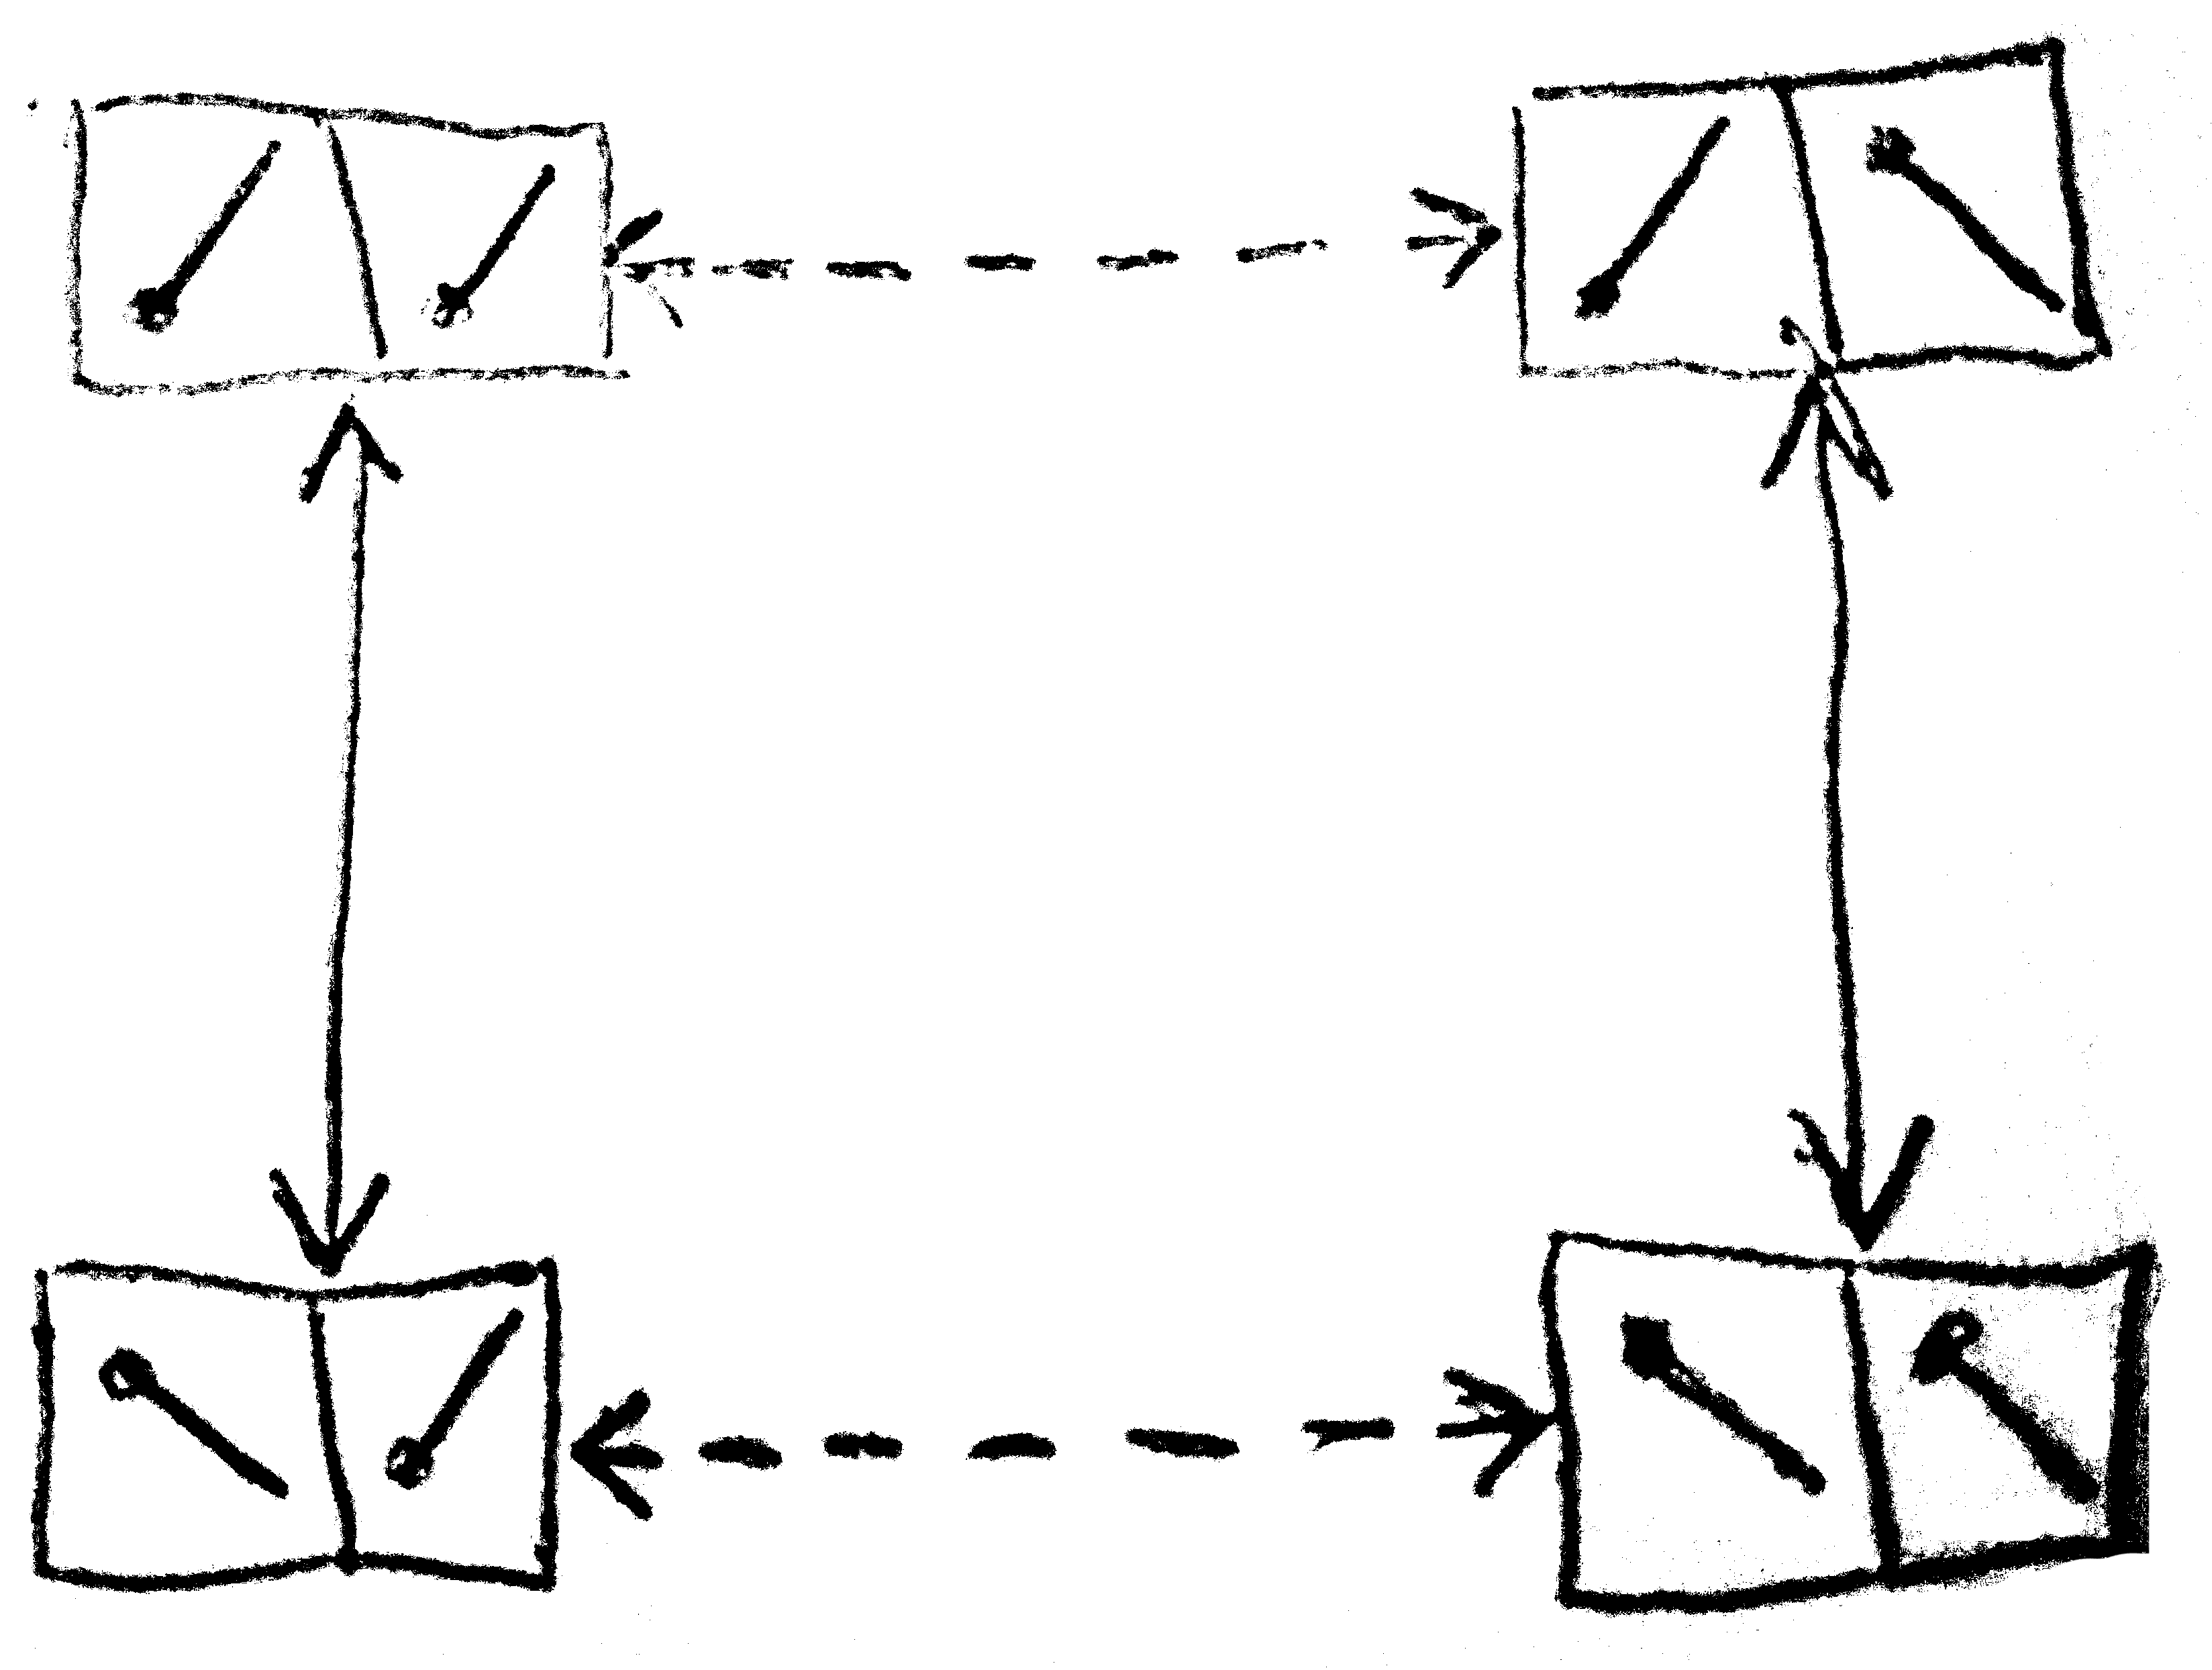
\includegraphics[width=7cm]{figure/two_switches.png}
\end{minipage}

\begin{enumerate}[start=11]
  \item Изобрази граф Кэли для группы двух монеток на столе.
  \item Изобрази граф Кэли для картин в квартире Садовского.
  \item Изобрази кусочек графа Кэли для группы прибавления целых чисел.
  \item Изобрази граф Кэли для группы переключателей, если образующими считать два действия: щёлкнуть левым и щёлкнуть обоими переключателями сразу.
  \item Придумай группы с данными графами Кэли:

  \begin{minipage}[c]{0.5\textwidth}
  \centering
          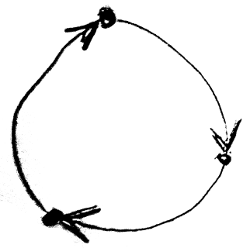
\includegraphics[width=5cm]{figure/c3b.png}
 \end{minipage}
 \begin{minipage}[c]{0.5\textwidth}
 \centering
         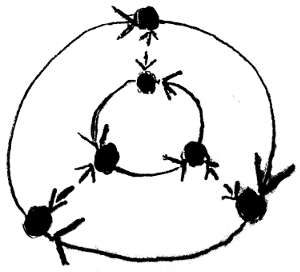
\includegraphics[width=5cm]{figure/s3b.png}
 \end{minipage}
  % \begin{minipage}{0.5\textwidth}
  %     \centering
  %     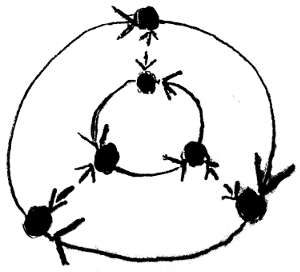
\includegraphics[width=0.3\linewidth, height=0.15\textheight]{figure/s3b.png}
  %     \captionof*{б)}
  % \end{minipage}

  %\item Чего больше: действий в группе или узлов на её графе Кэли?
  \item Можно ли сопоставить действия группы и вершины на графе Кэли? Если да, то как?
\end{enumerate}

Заметки: Были все школьники. Хорошо и легко зашёл граф Кэли. Можно сразу с него начинать. Сразу группа и её граф. Плохо: точно нужно больше явного перечисления элементов группы. Пожалуй, логичнее всего было бы начать с двух примеров с графом Кэли, полным списком элементов и списком образующих. Пример неабелевой группы: робот, даём ему инструкции вперед-назад, поворот. Лучше чем преобразования плоскости.

\newpage
\section{Группа симметрий}

\begin{enumerate}
  \item У Васи один носок надетый на левую ногу. Вася умеет выполнять следующие два образующих действия: «переодень носок на другую ногу» и «выверни носок наизнанку и переодень на другую ногу». Нарисуй граф Кэли. Сколько всего действий в данной группе?
  \item В вершинах квадрата стоят зондера в шапках. Шапки одинаковые, но одна вывернута наизнанку. Зондера умеют выполнять два образующих действия: передать шапки по часовой стрелке, вывернуть все шапки наоборот. Нарисуй граф Кэли. Сколько всего действий в данной группе?
  \item Солдат умеет выполнять одну образующую команду: «повернись на 90 градусов по часовой стрелке». Нарисуй граф Кэли. Сколько всего действий в данной группе?
\end{enumerate}



Определение. \textbf{Группа симметрий} — набор действий, переводящих фигуру (тело) ровно в себя и сохраняющий все расстояния между точками.

\begin{enumerate}[resume]
\item  Нарисуй граф Кэли для группы симметрий:
\begin{enumerate}
  \item прямоугольника с неравными сторонами;
  \item равнобедренного, но не равностороннего треугольника;
  \item равностороннего треугольника;
  \item квадрата;
  \item молекулы борной кислоты $B(OH)_3$ и молекулы этилена $C_2H_4$;


   \begin{minipage}[c]{0.5\textwidth}
   \centering
           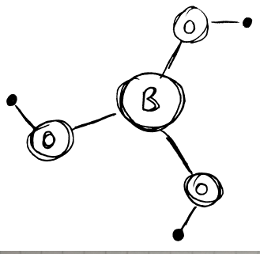
\includegraphics[width=5cm]{figure/boric_acidb.png}
   \end{minipage}
   \begin{minipage}[c]{0.5\textwidth}
   \centering
           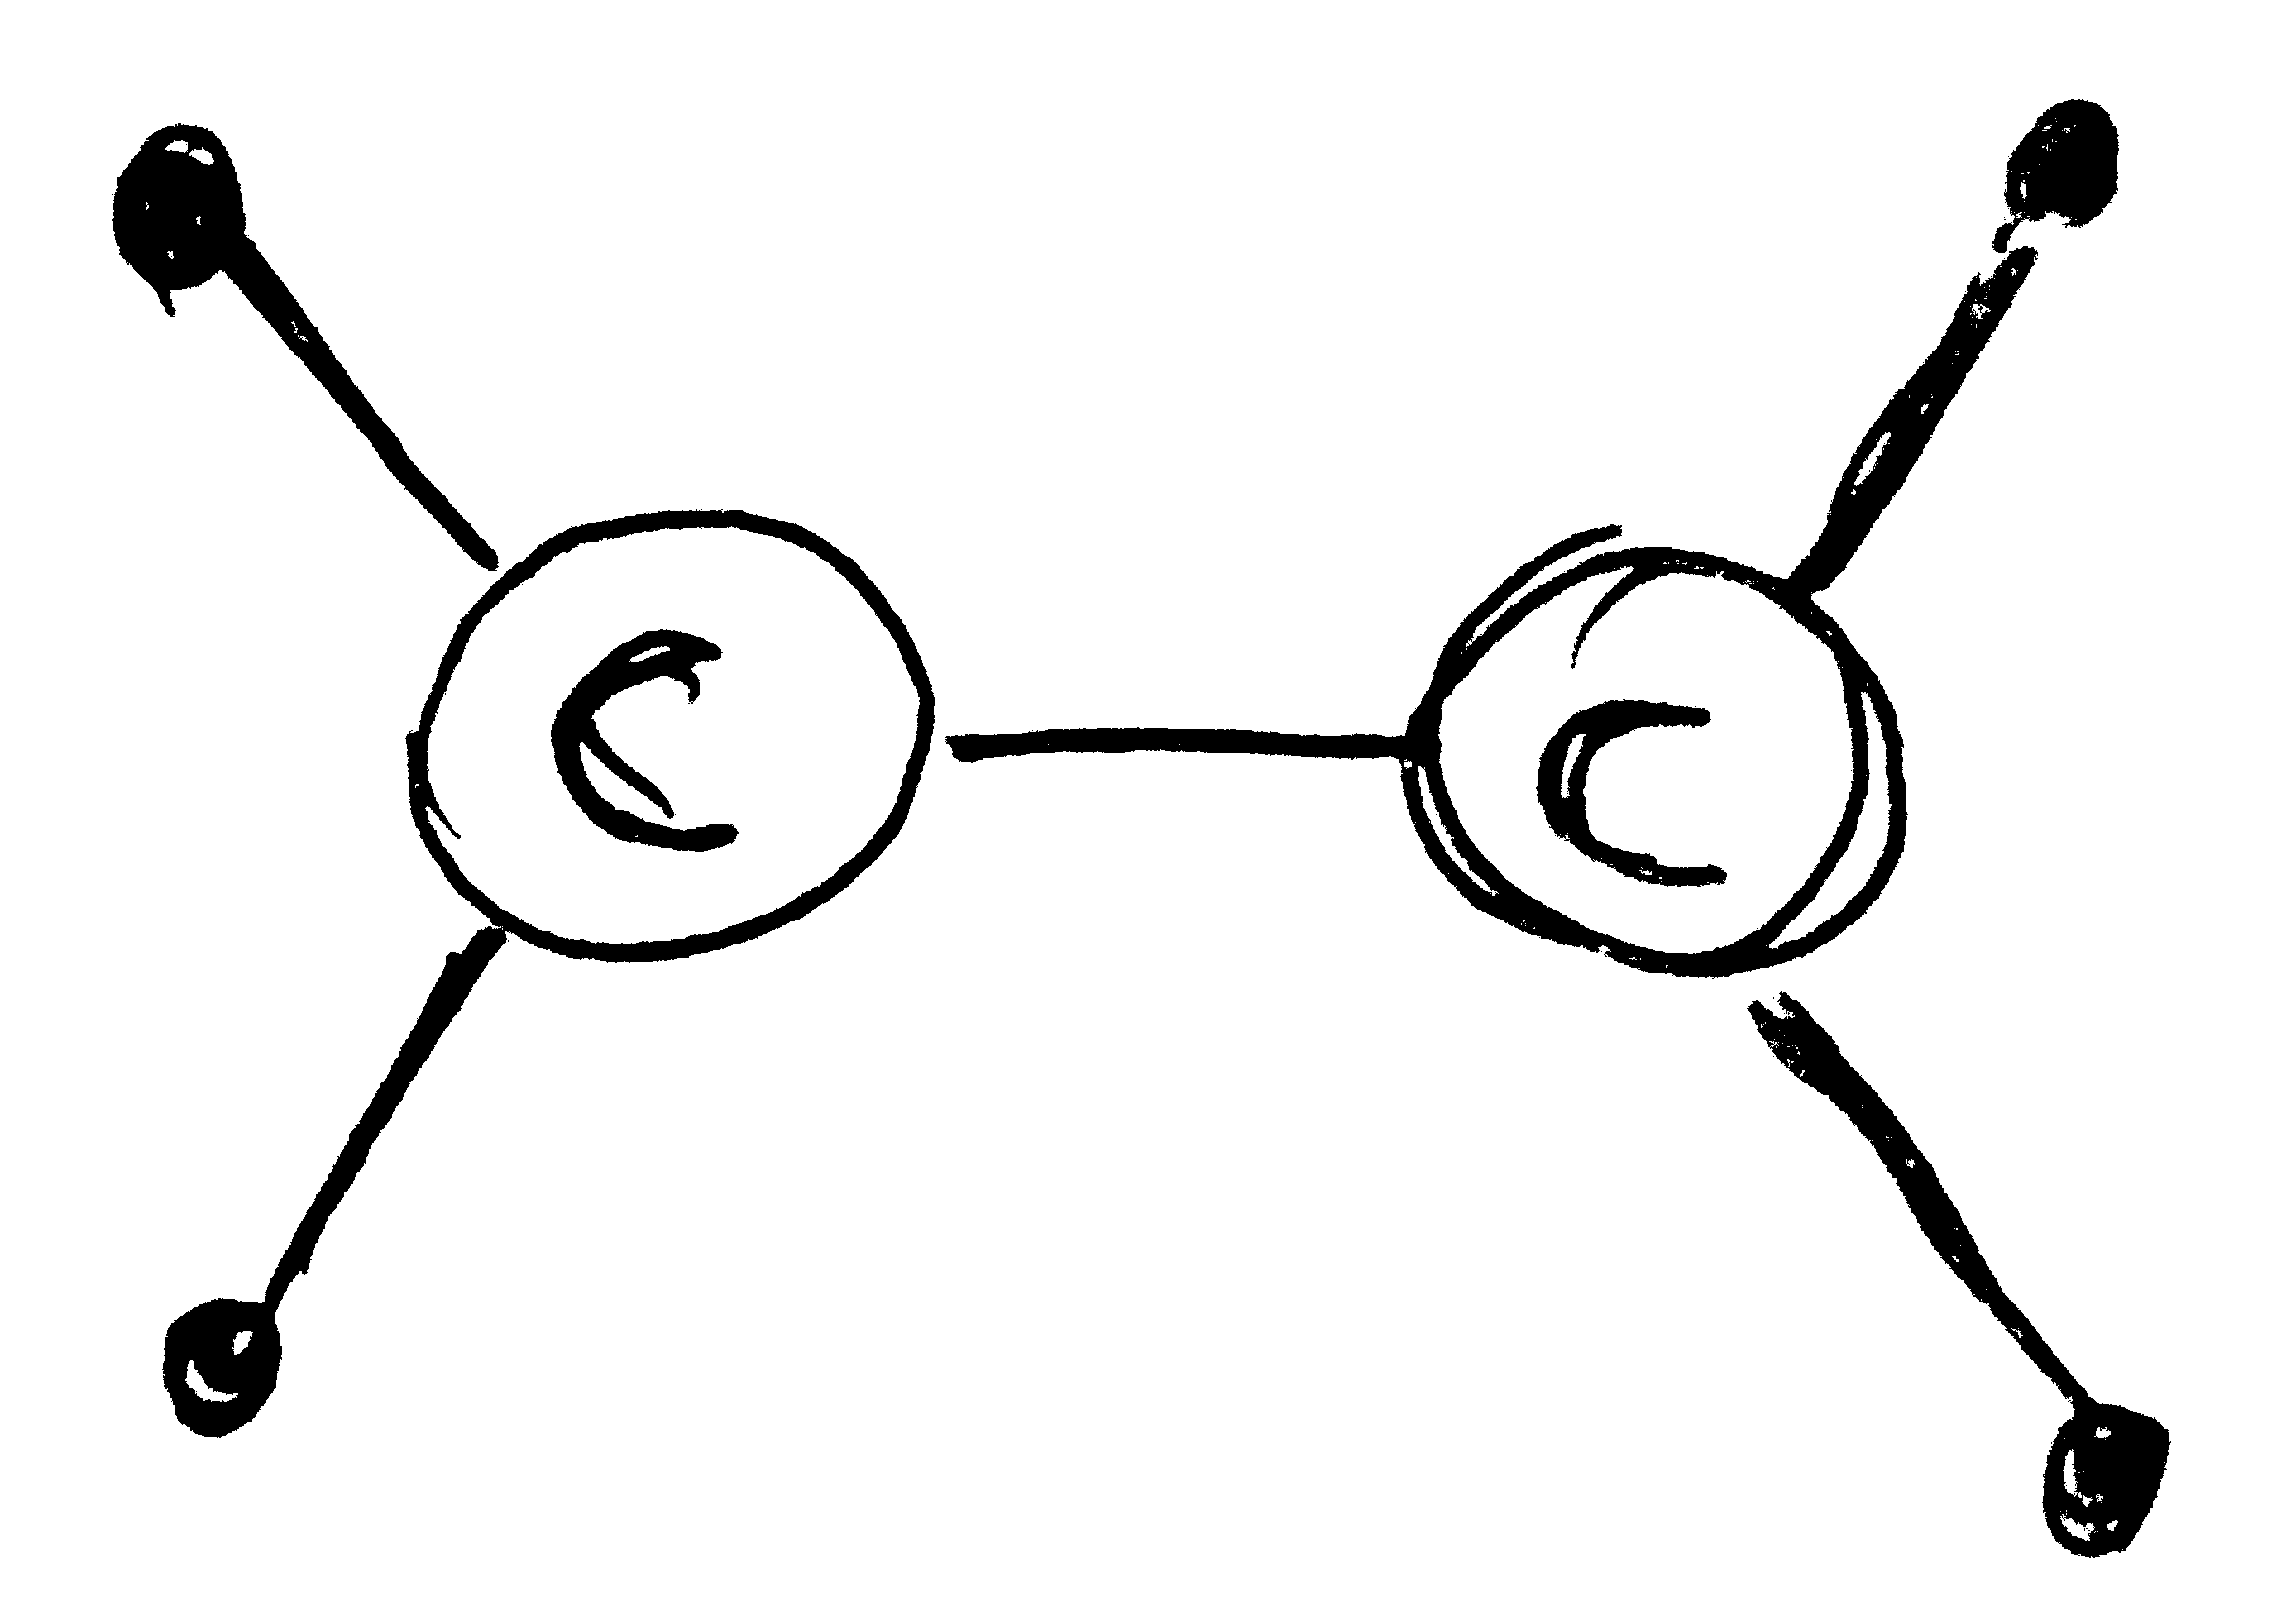
\includegraphics[width=5cm]{figure/ethylene.png}
   \end{minipage}


  \item мозаики;


  \begin{minipage}[c]{\textwidth}
  \centering
          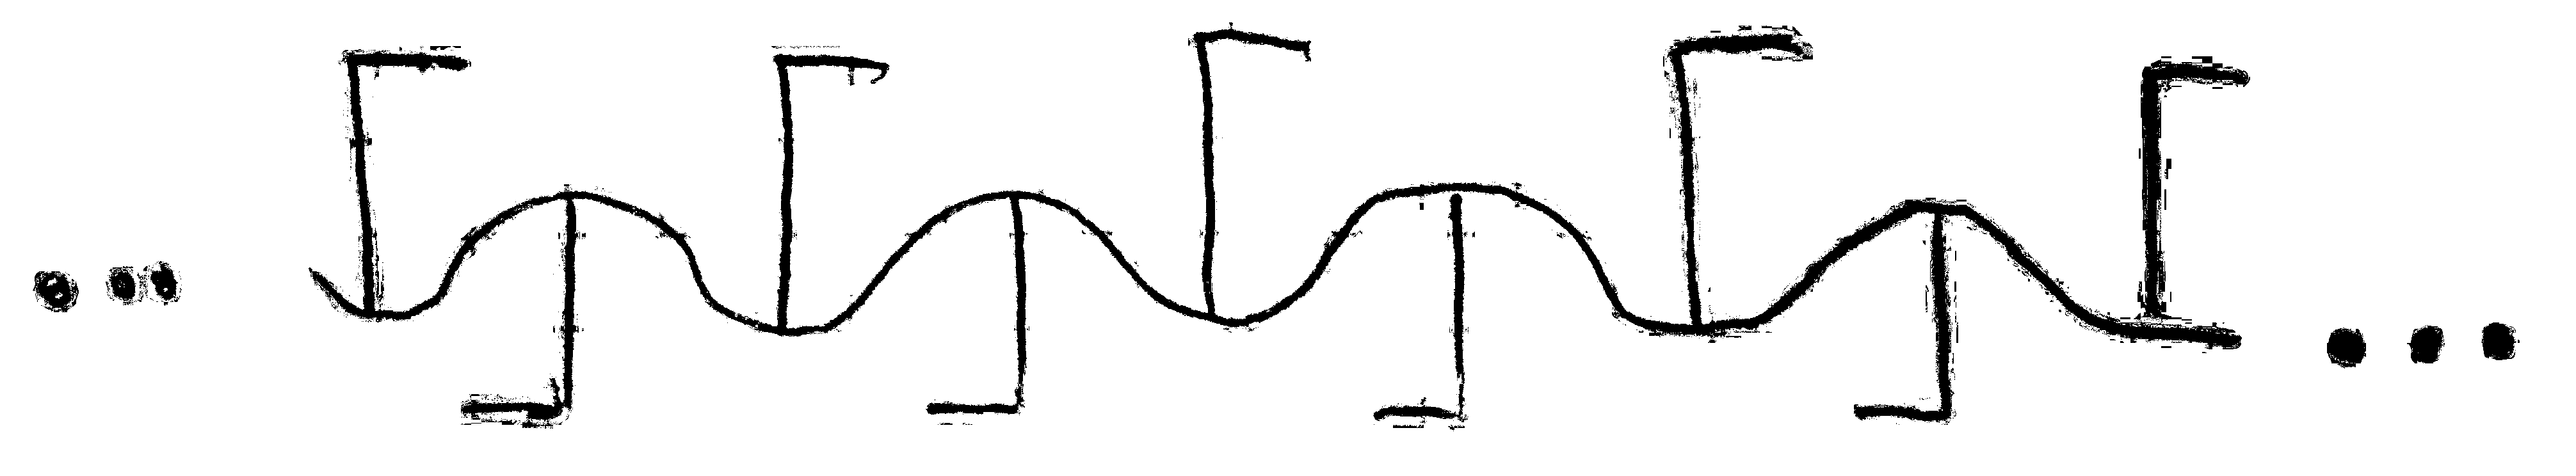
\includegraphics[width=10cm]{figure/mosaic_a.png}
  \end{minipage}


  \item мозаики;


  \begin{minipage}[c]{\textwidth}
  \centering
          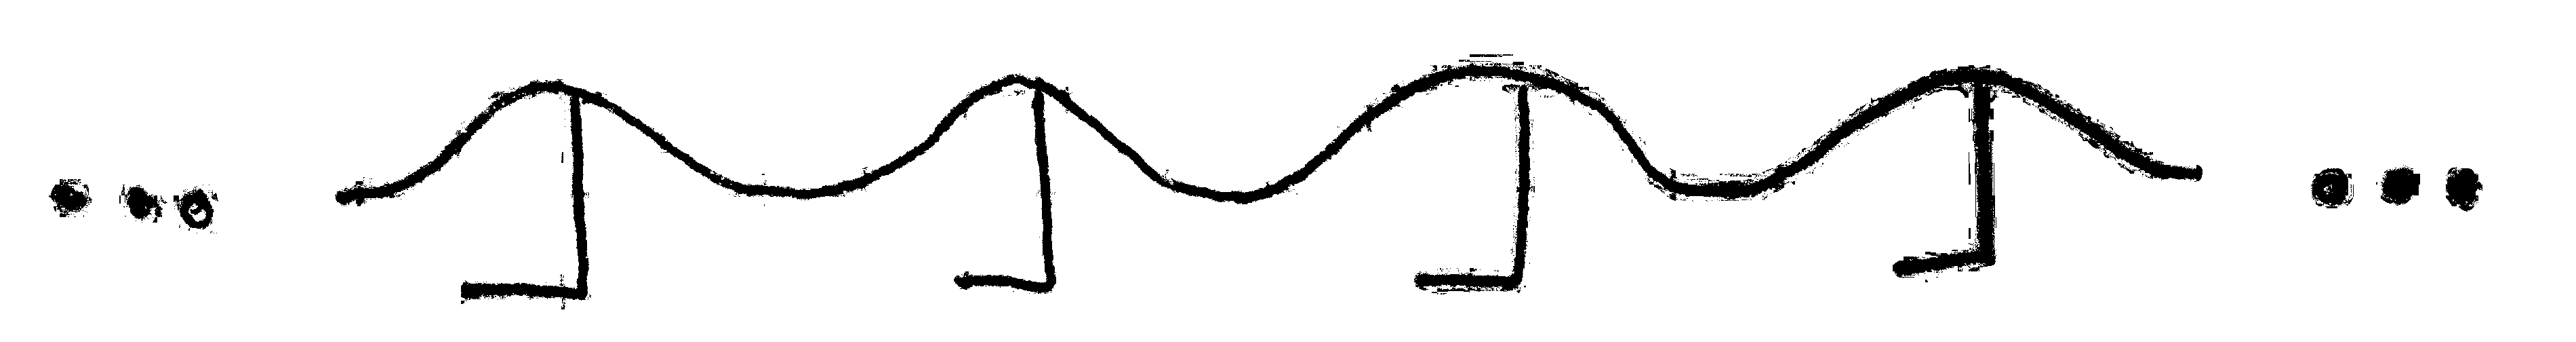
\includegraphics[width=10cm]{figure/mosaic_b.png}
  \end{minipage}


  \item мозаики;


  \begin{minipage}[c]{\textwidth}
  \centering
          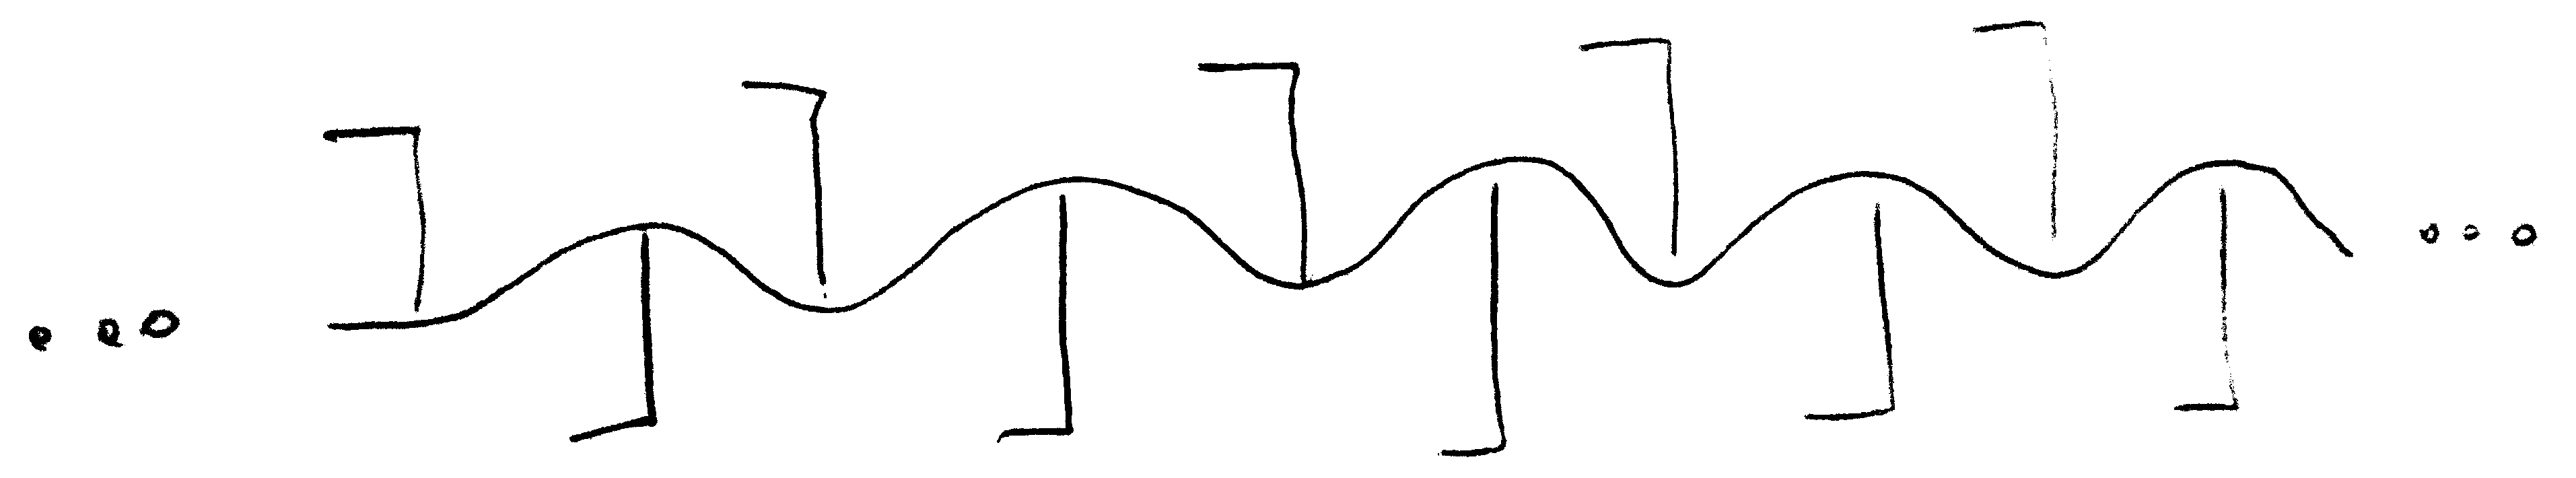
\includegraphics[width=10cm]{figure/mosaic_c.png}
  \end{minipage}


  \item мозаики;


  \begin{minipage}[c]{\textwidth}
  \centering
          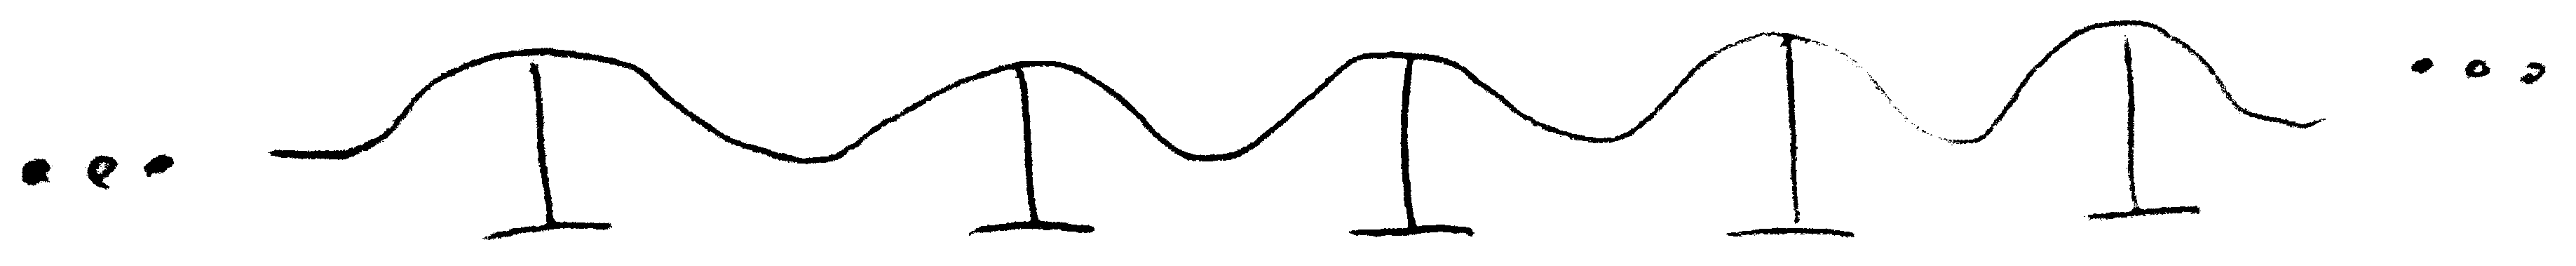
\includegraphics[width=10cm]{figure/mosaic_d.png}
  \end{minipage}

\end{enumerate}
\end{enumerate}


Все были. Сначала сделали первобытные спиннеры («вертушки»). Нужен лист бумаги и кнопка. Построили граф Кэли группы симметрий вертушки. Явно выписали полный список группы. Далее школьники решали задачи. Илья представил задачу с симметриями прямоугольника. На столе под присмотром Сони часть школьников залезла в таблицы умножения.

\newpage
\section{Таблица умножения}

Наглядное определение. \textbf{Таблица умножения}. В строке $r$ в столбце $c$ находится произведение $r * c$.

\begin{minipage}[c]{\textwidth}
\centering
        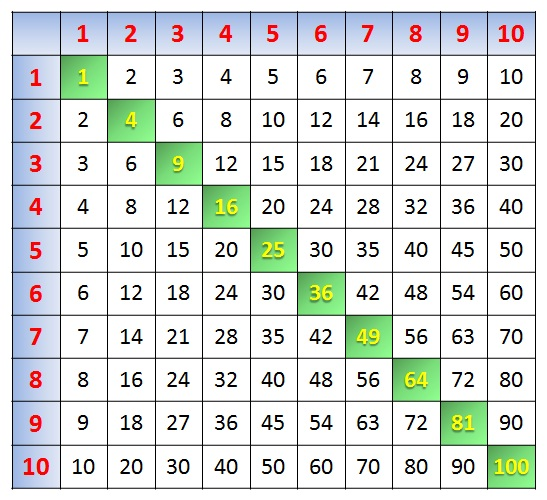
\includegraphics[width=5cm]{figure/table_mult.jpeg}
\end{minipage}

\begin{enumerate}[resume]

\item Составь таблицы умножения для групп:

\begin{enumerate}
    \item Группа Клейна. При входе в ВК два выключателя. Зондер умеет выполнять два образующих действия: щёлкать левым выключателем и щёлкать правым.
    \item «Вращение солдата» (группа симметрий «вертушки»). Солдат умеет выполнять одну образующую команду: «повернись на 90 градусов по часовой стрелке».
    \item «Переодевание носка». У Васи один носок надетый на левую ногу. Вася умеет выполнять следующие два образующих действия: «переодень носок на другую ногу» и «выверни носок наизнанку и переодень на другую ногу».
    \item Группа симметрий равнобедренного треугольника.
    \item Группа симметрий равностороннего треугольника.
    \item Группа симметрий квадрата.
    \item молекулы борной кислоты $B(OH)_3$ и молекулы этилена $C_2H_4$;


     \begin{minipage}[c]{0.5\textwidth}
     \centering
             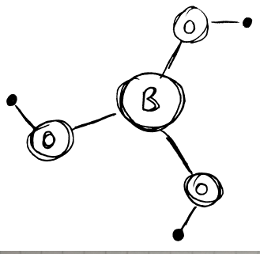
\includegraphics[width=5cm]{figure/boric_acidb.png}
     \end{minipage}
     \begin{minipage}[c]{0.5\textwidth}
     \centering
             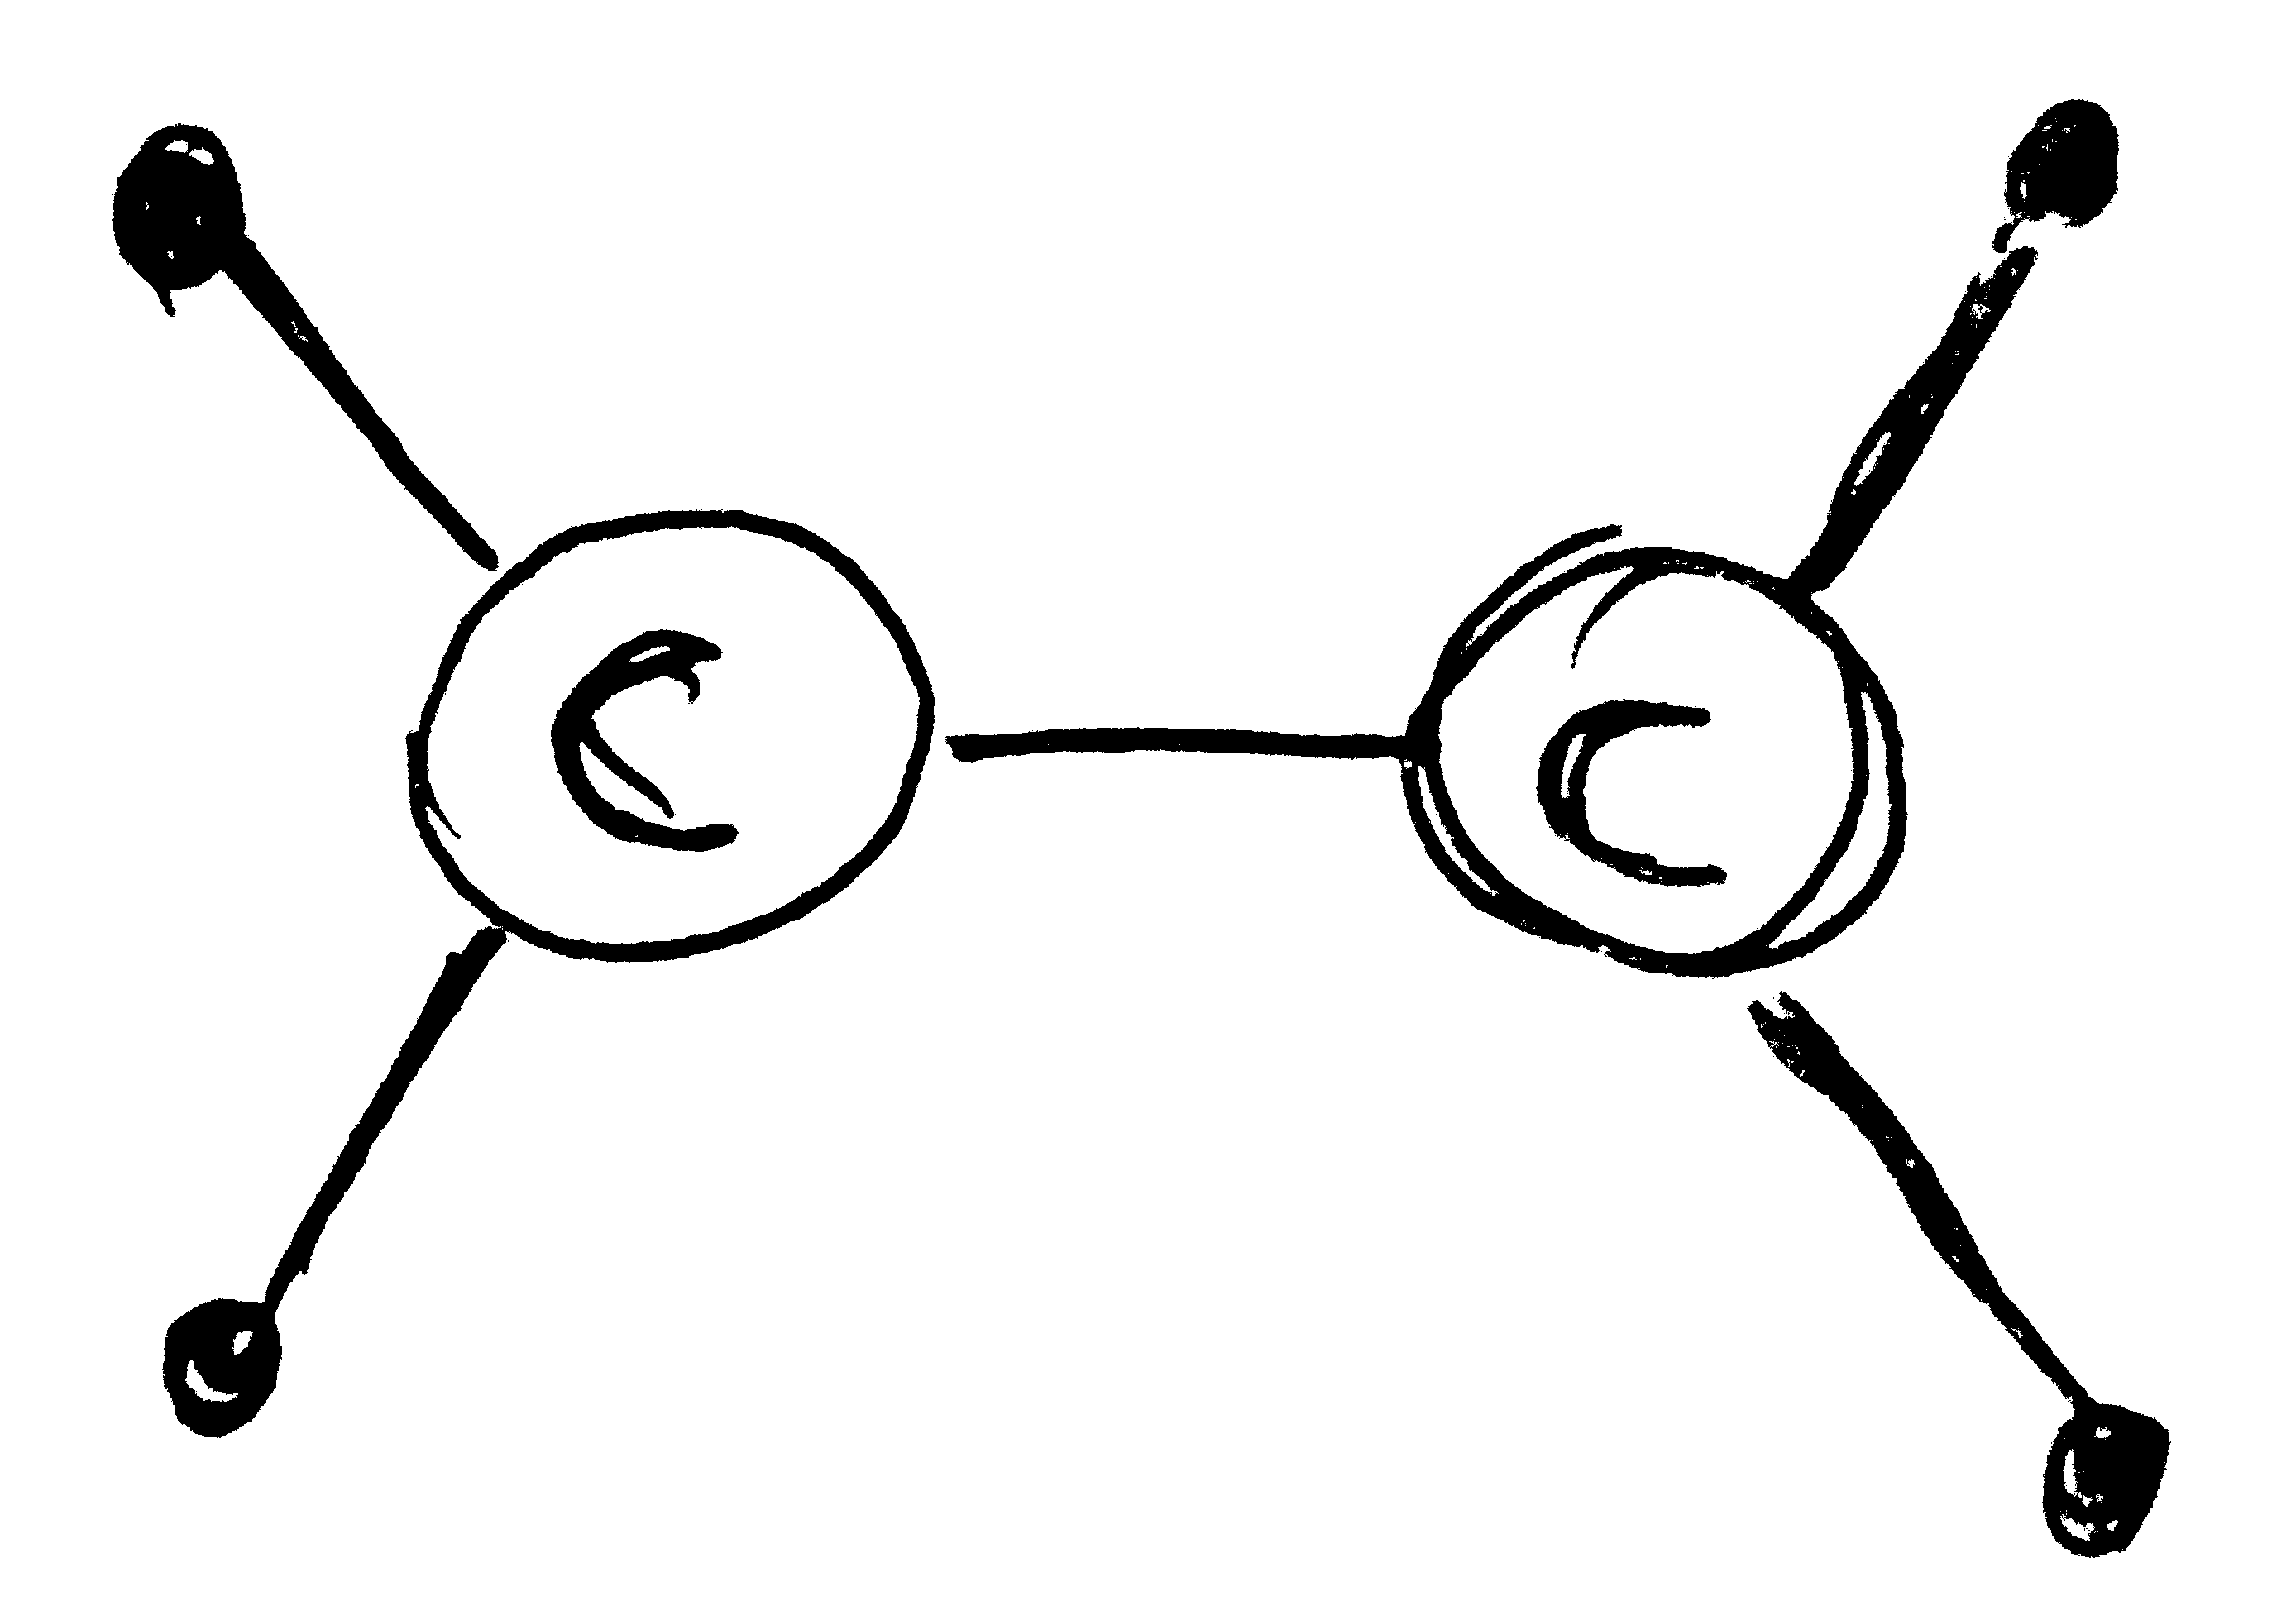
\includegraphics[width=5cm]{figure/ethylene.png}
     \end{minipage}

\end{enumerate}

\item Почему в таблице умножения в одной строке (или в столбце) все результаты различны?

\item Дозаполни все таблицы умножения. Буква $e$ означает действие «ничего не делать».


  \begin{minipage}[c]{\textwidth}
  \centering
  а)
  \begin{tabular}{c|c|c|}
       & $e$ & $a$  \\
  \midrule
  $e$  &     &      \\
  \midrule
  $a$  &     &      \\
  \midrule
  \end{tabular};
  \;
  б)
  \begin{tabular}{c|c|c|c}
       & $e$ & $a$ & $b$\\
  \midrule
  $e$  &     &    &  \\
  \midrule
  $a$  &     &    &  \\
  \midrule
  $b$  &     &    &  \\
  \midrule
  \end{tabular}
  \;
  в)
  \begin{tabular}{c|c|c|c|c}
       & $e$ & $a$ & $b$ & $c$ \\
  \midrule
  $e$  &     &    &   & \\
  \midrule
  $a$  &     & $b$ &   &  \\
  \midrule
  $b$  &     &    &   &  \\
  \midrule
  $c$  &     &    &   &  \\
  \midrule
  \end{tabular}
  \end{minipage}

\end{enumerate}

Определение. Группа действий называется \textbf{абелевой} (коммутативной), если порядок выполнения действий не влияет на результат, $a * b = b * a$.

Формальное определение группы. Множество $G$ с операцией-тирьямпампацией $*$ называется группой, если:
\begin{enumerate}
  \item[G1.] В множестве $G$ существует «единичный» элемент, $e$, такой что для всех $g$ выполнено $e*g=g*e=g$.
  \item[G2.] Для любого элемента $g \in G$ существует обратный элемент, $g^{-1}$, такой что $g^{-1}*g=g*g^{-1}=e$.
  \item[G3.] Операция-тирьямпампация $*$ ассоциативна, то есть для любых $a$, $b$, $c$ выполнено $(a * b) * c = a * (b * c)$.
\end{enumerate}

Пример. Ним-сложение натуральных чисел с нулём. Тирьямпампацию $*$ делаем так: каждое слагаемое переводим в двоичную систему счисления, складываем числа столбиком по принципу $0+0=1+1=0$, $1+0=0+1=1$, переводим из двоичной обратно.

\begin{enumerate}[start=4]
  \item Сделай ним-сложения: $2 * 6$, $3 * 9$, $3 * 7$.
  \item Что является «единицей» в ним-сложении?
  \item Найди обратные элементы: $6^{-1}$, $5^{-1}$.
\end{enumerate}

Рассказ про игру ним. Школьники играют две партии по парам.

Теорема. Позиция в игре ним является выигрышной, если ним-сумма строго больше нуля.

Выигрышная стратегия: подсунь противнику ним-сумму равную нулю.

Играю по ним-стратегии против добровольца Ильи.

\newpage
\section{Примеры групп и глубже про ним-сумму}

\begin{enumerate}
\item Зондер надел сначала рубашку, а затем свитер, поэтому, чтобы ему раздеться надо сначала снять свитер, а потом — рубашку. Запиши это утверждение\footnote{Здесь не совсем группа, так как невозможно снять свитер, когда он не надет, но получаемое тождество выполнено в любой группе.} с помощью действий $a$ и $b$, где $a$ — «надеть свитер», а $b$ — «надеть рубашку».

\todo[inline]{это упражнение надо переставить на после задания группы системой образующих и соотношений. Переформулировать!}
\item Какие множества являются группой? Абелевой группой? Если множество — группа, то поясни, что является единицей группы и что является обратным элементом.
\todo[inline]{оформить каждое упражнение отдельно. сначала спросить выполнить пару операций. потом спросить, что такое $e$...}
\begin{enumerate}
\item Рациональные числа. Под тирьямпампацией $*$ понимается обычное сложение.
\item Рациональные числа. Под тирьямпампацией $*$ понимается обычное умножение.
\item Рациональные числа кроме нуля. Под тирьямпампацией $*$ понимается обычное умножение.
\item Множество $G$ — натуральные числа и ноль. Под тирьямпампацией $*$ понимается ним-сложение.
\item Множество $G$ — скорости от минус до плюс скорости света. Тирьямпампация $*$ делается так
\[
a * b = \frac{a + b}{1 + ab/c^2},
\]
где $c$ — скорость света. Найди $0.5c * 0.5c$, $0.5c * 0.7c$, $-0.9c * 0.5c$.

\end{enumerate}
\end{enumerate}

Игры :) Рассмотрим игры, где у игроков одинаковое множество ходов. Например, шахматы не подходят.


\begin{enumerate}

\item Игра: двигай фишку по графу.

\begin{minipage}[c]{0.5\textwidth}
\centering
        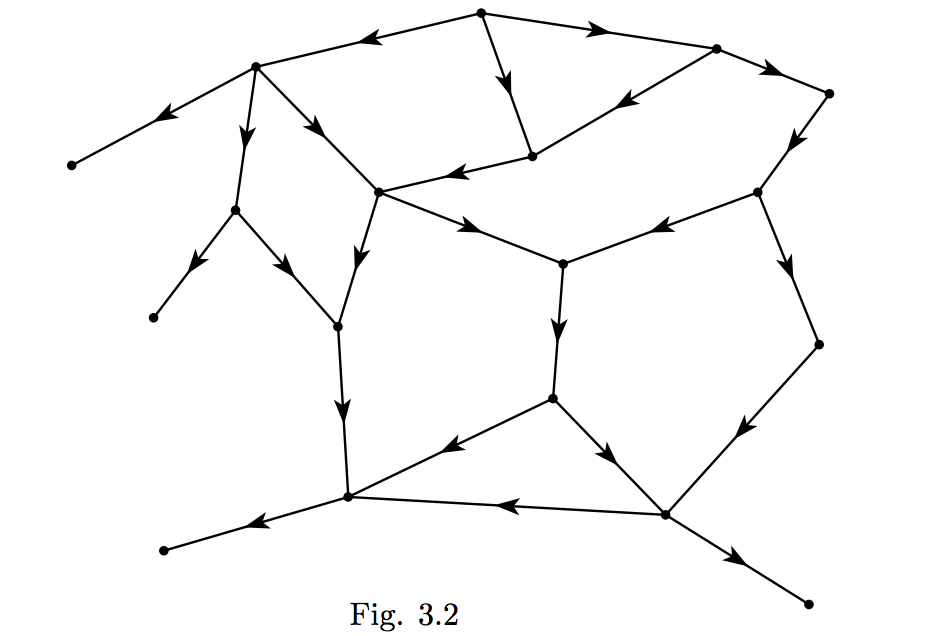
\includegraphics[width=9cm]{figure/game_a.png}
\end{minipage}
\begin{minipage}[c]{0.5\textwidth}
\centering
        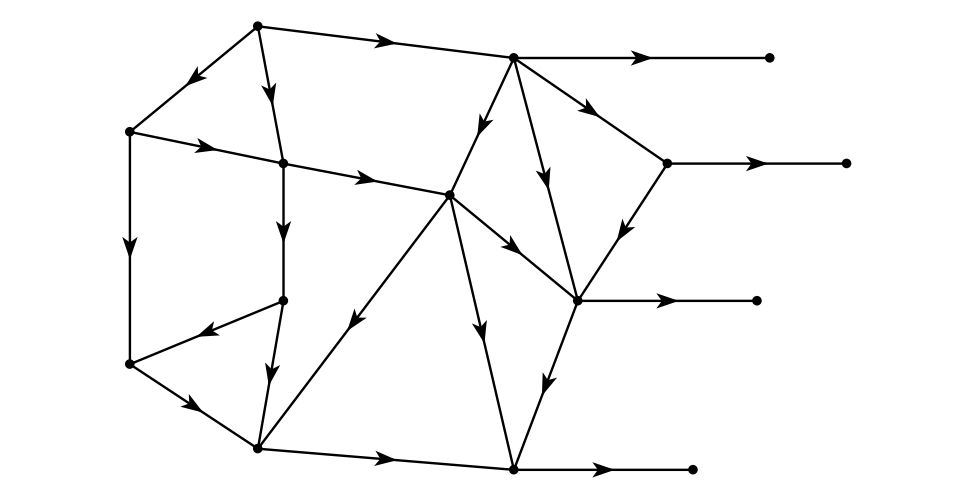
\includegraphics[width=9cm]{figure/game_b.png}
\end{minipage}

\item Игра: переворачивай черепах! Переверни $H\to T$ и любую монетку слева от перевернутой по желанию.

   a)   H-T-T-H-T-T-H    б)  T-H-H-T-T-H

\item Автомобильная пробка. Монетки на дорожке ведущей в пробку справа. Обгонять нельзя, можно ходить на любое число ходов в сторону пробки одной монеткой.

   а) M - - - M - - M - - - M - - |    б) M - M - M - - M - - - M - - - - |

\item Определение. Ним-стоимостью позиции, $nim(G)$, называется минимальное неотрицательное число, не входящее в ним-стоимости позиций, следующих за позицией $G$. Рассчитайте ним-стоимости позиций в игре с графом.



\end{enumerate}

%Теорема. В играх, где у игроков одинаковые доступные ходы, позиция является выигрышной если и только если её ним-стоимость положительна.



% Доказательство. %За выигрышной позицией следуют только проигрышные. За проигрышной позицией есть хотя бы одна выигрышная. Положительность ним-суммы подчиняется этим же свойствам.
\newpage
\section{Великое примирение и сумма игр}

\subsection{Великое примерение!}

Определение. Множество $G$ с операцией $*$ — группа, если
\begin{enumerate}
  \item[A1.] Результат операции $a * b$ определён для всех $a$ и $b$ и всегда лежит внутри $G$.
  \item[A2.] Есть нейтральный элемент $e$, такой что $a*e=e*a=a$ для всех $a$.
  \item[A3.] У любого элемента $a$ есть обратный $a^{-1}$, такой что $a*a^{-1}=a^{-1}*a=e$.
  \item[A4.] Операция $a * b$ ассоциативна, то есть для любых $a$, $b$ и $c$ выполнено равенство $a * (b * c) = (a * b) * c$.
\end{enumerate}

\begin{enumerate}
  \item Рассмотрим обычные действительные числа. Какие свойства группы нарушает действие $a * b = 2a + 2b$?
  \item Рассмотрим действительные числа. Какие свойства группы нарушает действие $a * b = a - b$?
\end{enumerate}


Летнешкольное определение. \textbf{Группа} (group) — набор действий, обладающий следующими свойствами:
\begin{enumerate}
  \item[G1.] Есть фиксированный список образующих действий, с помощью которых можно получить остальные действия.
  \item[G2.] Действия являются детерминистическими.
  \item[G3.] У любого действия есть обратное действие.
  \item[G4.] Действия можно осуществлять в любом порядке в любом количестве и при этом получается некое действие.
\end{enumerate}


Примиряем летнешкольное определение группы и формальное определение.

\begin{enumerate}[resume]
\item Что в летнешкольком определении является элементом группы?
\item Что в летнешкольком определением является операцией $*$?
\item Какое действие в летнешкольном определении является единицей?
\item Почему в летнешкольном определении группы выполнена ассоциативность?
\item Почему группа в летнешкольном определении является формальной группой?
\item Почему формальная группа является группой в летнешкольном определении?
\end{enumerate}

\subsection{Складываем игры}

Сумма игр $G_1 * G_2$ — это игра, в которой игрок при ходе выбирает одну из игр, $G_1$ или $G_2$, и делает в ней ход по её правилам.

Пример. Складываем два графа.

\begin{enumerate}
  \item Какая игра получится если сложить ним с кучками 3-2-7 и ним кучками 2-8?
  \item Сложите два графа $G_1$ и $G_2$:
  \begin{minipage}[c]{0.5\textwidth}
  \centering
          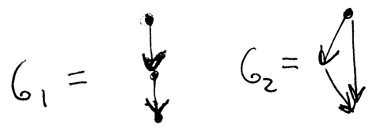
\includegraphics[width=9cm]{figure/graph_sum.png}
  \end{minipage}

  \item Найдите ним-стоимость позиций игры $G_1$, позиций игры $G_2$ и позиций игры $G = G_1 + G_2$.
\end{enumerate}



Теорема (Шпраг-Гранди, Sprague-Grundy):
\[
nim(G_1 * G_2) = nim(G_1) \oplus nim(G_2),
\]
где $*$ — сложение игр, а $\oplus$ — сложение ним-чисел.

Определение. Будем считать две игры идентичными, если у них одинаковая ним-стоимость.

\begin{enumerate}
  \item Идентичны ли ним с кучками 2-6-9 и кучками 5-9-1?
  \item Упрости ним-стоимости $nim(G * G)$, $nim(G * G * G)$
  \item Что является единицей группы игр?
  \item Что такое игра, обратная к данной?
  \item Верно ли, что $G_1 * G_2 = G_2 * G_1$?
\end{enumerate}


Решаем черепашек и машинки.

\begin{enumerate}
  \item Найдите оптимальный ход в сумме игр

  \begin{minipage}[c]{0.5\textwidth}
  \centering
          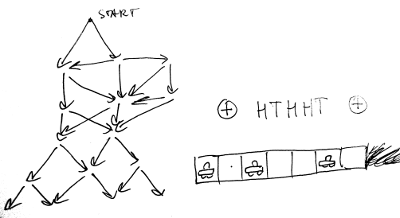
\includegraphics[width=16cm]{figure/game_sum.png}
  \end{minipage}

\end{enumerate}


При решении машинок я ошибся и перепутал нечётные интервала с начала и с конца.



\newpage

\section{Группа перестановок}

\subsection{Работа над ошибками :)}

Найдите оптимальный ход в сумме игр

\begin{minipage}[c]{0.5\textwidth}
\centering
        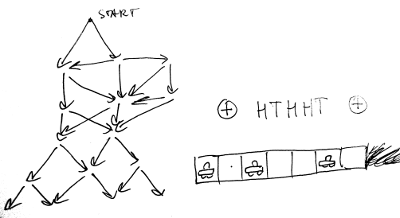
\includegraphics[width=16cm]{figure/game_sum.png}
\end{minipage}

\subsection{Группа перестановок}

Определение. \textbf{Группа перестановок} (подстановок) $n$ предметов, $S_n$. Другое название: симметрическая группа.

Обозначения на примерах:

Перестановка, переводящая $1\to 2$, $2\to 4$, $3\to 1$, $4\to 3$, записывается так:
\[
\begin{pmatrix}
  1 & 2 & 3 & 4 \\
  2 & 4 & 1 & 3 \\
\end{pmatrix}
\]

Образ: представь себе школьников, сидящих на занумерованных стульях. Перестановка говорит с какого стула (первая строка) на какой стул (вторая строка) надо пересаживаться школьникам.

Определение. \textbf{Циклом} $(2567)$ называется перестановка, переводящая $2\to 5$, $5 \to 6$, $6\to 7$, $7\to 2$, и оставляющая другие числа на своих местах. Например,
\[
(2567) =
\begin{pmatrix}
1 & 2 & 3 & 4 & 5 & 6 & 7 \\
1 & 5 & 3 & 4 & 6 & 7 & 2 \\
\end{pmatrix}.
\]

Определение. Цикл из двух элементов, например, $(49)$, называется \textbf{транспозицией}.

Под умножением циклов подразумевается их последовательное применение.

\begin{enumerate}
\item Перемножь циклы $(2541)\circ(123)\circ(124)$.
\item Рассмотрим перестановку
\[
\sigma = \begin{pmatrix}
  1 & 2 & 3 & 4 & 5 \\
  4 & 5 & 1 & 3 & 2 \\
\end{pmatrix}.
\]
Разложи перестановку в произведение непересекающихся циклов.

Подсказка: нарисуй стрелочками с какого на какой стул пересаживаются школьники.
\end{enumerate}

\newpage
\section{Группа перестановок-2}

Определение. \textbf{Группа перестановок} (подстановок) $n$ предметов, $S_n$. Другое название: симметрическая группа.

Обозначения на примерах:

Перестановка, переводящая $1\to 2$, $2\to 4$, $3\to 1$, $4\to 3$, записывается так:
\[
\begin{pmatrix}
  1 & 2 & 3 & 4 \\
  2 & 4 & 1 & 3 \\
\end{pmatrix}
\]

Образ: представь себе школьников, сидящих на занумерованных стульях. Перестановка говорит с какого стула (первая строка) на какой стул (вторая строка) надо пересаживаться школьникам.

Определение. \textbf{Циклом} $(2567)$ называется перестановка, переводящая $2\to 5$, $5 \to 6$, $6\to 7$, $7\to 2$, и оставляющая другие числа на своих местах. Например,
\[
(2567) =
\begin{pmatrix}
1 & 2 & 3 & 4 & 5 & 6 & 7 \\
1 & 5 & 3 & 4 & 6 & 7 & 2 \\
\end{pmatrix}.
\]

Определение. Цикл из двух элементов, например, $(49)$, называется \textbf{транспозицией}.

Под умножением циклов подразумевается их последовательное применение.

\begin{enumerate}
\item Найди все циклы совпадающие с $(159)$.
\item Может ли во второй строке перестановки стоять два одинаковых числа?
\item Докажи, что любую перестановку можно разложить в произведение циклов.
\item Разложи цикл $(14532)$ в произведение транспозиций.
\item Докажи, что любой цикл можно разложить в произведение транспозиций.
\item Нарисуй граф Кэли группы $S_3$ взяв за образующие $(12)$ и $(23)$.
\item Нарисуй граф Кэли группы $S_3$ взяв за образующие $(12)$ и $(123)$.
\item Похожа ли группа $S_3$ на группу симметрий равностороннего треугольника?
\item Найди перестановку обратную следующей:
\[
    \begin{pmatrix}
        1& 2& 3& 4& 5& 6 \\
        3& 1& 6& 4& 2& 5 \\
    \end{pmatrix}
\]
\item Предложи два разных разложения цикла $(1234)$ на транспозиции.
\item В классе 17 школьников сидят на 17-ти занумерованных стульях. Учитель требует, чтобы школьники пересаживались каждую минуту по следующему правилу:
\setcounter{MaxMatrixCols}{20} % по дефолту pmatrix позволяет 20 колонок
\[
    \begin{pmatrix}
  1 & 2 & 3 & 4 & 5 & 6 & 7 & 8 & 9 & 10 & 11 & 12 & 13 & 14 & 15 & 16 & 17 \\
  3 & 5 &10 & 8 &11 & 14& 15& 6 & 13& 1  &  4 &  9 & 7  &  2 & 12 & 17 & 16 \\
  \end{pmatrix}
\]
Через сколько минут все школьники вернутся на свои первоначальные места?
\end{enumerate}

Определение. Наименьшее количество раз, которое нужно повторить перестановку $s$, чтобы получилась исходная расстановка чисел, называется \textbf{порядком перестановки} $s$.

\begin{enumerate}[resume]
\item Найди порядок перестановок $a=(12784)$ и $b=(12)(456)$.
\item В группе $S_{9}$ приведи пример перестановки порядка $7$, $10$, $12$, $11$, если они существуют.
\item Зондер утверждает, что разложил некую перестановку $\sigma$ на транспозиции двумя способами: на 13 транспозиций и на 42 транспозиции. Возможно ли такое?
\end{enumerate}

Определение. Перестановка $\sigma$ из $S_n$ называется \textbf{чётной}, если она раскладывается в чётное количество транспозиций.

\begin{enumerate}[resume]
  \item Определи, являются ли чётными перестановки:
  \begin{enumerate}
    \item $\alpha = (12345)$;
    \item $\beta = (5732)$;
    \item $\gamma = (234)\circ(5678)$.
  \end{enumerate}

  \item Разрешима ли на кубике Рубика позиция, где переставлены два угловых кубика? А два бортовых кубика?
  \item Разрешима ли в игре «15» позиция, где переставлены 1 и 2? А 14 и 15?
  \item На одном старом телефоне я видел такую игрушку. В вершинах квадрата $ABCD$ лежат шарики разных цветов. Нажав на любую вершину игрок может переставить циклом шарики в этой вершине и двух соседних. Можно ли в этой игрушке переставить шарики в двух соседних вершинах квадрата?
\end{enumerate}


\newpage
\section{Частые гости}

Определение. Рассмотрим некоторую перестановку $a$, которая пересаживает школьников по стульям. Если до перестановки $a$ Вася сидел раньше Пети, а после перестановки — позже, то назовём это беспорядком.

Число беспорядков легко увидеть на диаграмме. Рассмотрим цикл $(143)$:

\begin{minipage}[c]{0.5\textwidth}
  \centering
          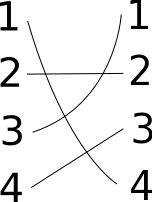
\includegraphics[width=4cm]{figure/swap_number.png}
  \end{minipage}


Цикл создаёт 4 беспорядка\footnote{Линии следует проводить так, чтобы избегать пересечений в одной точке!}.

\begin{enumerate}
\item Изначально все школьники сидят на стульях в алфавитном порядке. Сколько беспорядков создаёт транспозиция $(39)$? А сколько беспорядков создаёт цикл $(572)$?
\item Перестановка $a$ сама по себе создаёт 8 беспорядков, перестановка $b$ сама по себе — $7$ беспорядков. Сколько беспорядков может создавать перестановка $c=a\circ b$?
\item Какая перестановка получится, если за чётной перестановкой сделать нечётную?
\item Определи, являются ли чётными перестановки:
  \begin{enumerate}
    \item $\alpha = (12345)$;
    \item $\beta = (5732)$;
    \item $\gamma = (234)\circ(5678)$.
  \end{enumerate}
\item Цикл длиной 42 является чётной перестановкой или нечётной?
\item Разрешима ли на кубике Рубика позиция, где переставлены два угловых кубика? А два бортовых кубика?

\begin{minipage}[c]{0.5\textwidth}
\centering
        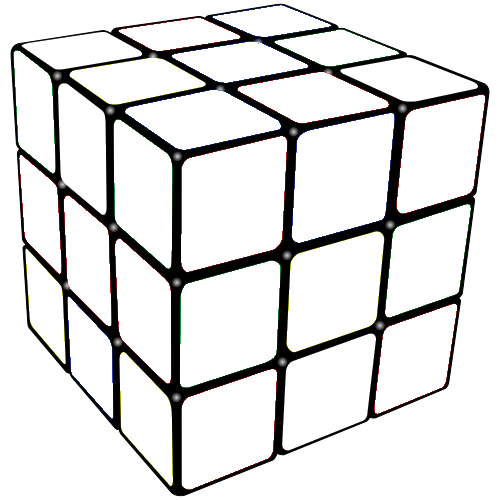
\includegraphics[width=4cm]{figure/rubik_cube.png}
\end{minipage}

\item Разрешима ли в игре «15» позиция, где переставлены 14 и 15? А 1 и 2?

\begin{minipage}[c]{0.5\textwidth}
\centering
        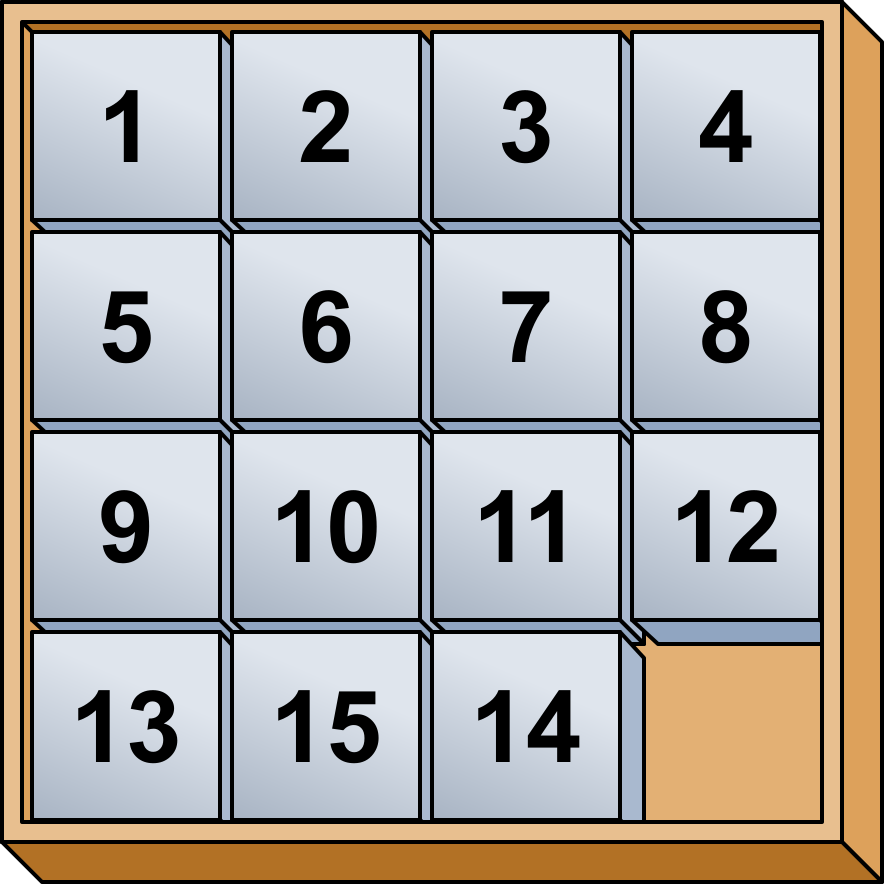
\includegraphics[width=4cm]{figure/15-puzzle-loyd.png}
\end{minipage}
\item На одном старом телефоне я видел такую игрушку. В вершинах квадрата $ABCD$ лежат шарики разных цветов. Нажав на любую вершину игрок может переставить циклом шарики в этой вершине и двух соседних. Можно ли в этой игрушке переставить шарики в двух соседних вершинах квадрата?
\end{enumerate}

Определение. \textbf{Тривиальной} называется группа состоящая из одного элемента, $\{e\}$.


Определение. \textbf{Циклическая группа порядка $n$} — группа симметрий классической детской $n$-угольной вертушки. Обозначение: $C_n$ или $\ZZ/n\ZZ$.

\begin{enumerate}[resume]
  \item Нарисуй граф Кэли групп $C_3$ и $C_4$.
\end{enumerate}

Определение. \textbf{Подгруппа} $H$ — часть группы $G$, которая сама по себе является группой. Обозначение $H<G$.

\begin{enumerate}[resume]
\item Выпиши все подгруппы в группе $V_4$ (действия зондера над двумя выключателями в ВК).
\item Выпиши все подгруппы в группе $S_3$ (перестановки трёх предметов).
\item Выпиши все подгруппы в группе $C_5$.
\item Выпиши все подгруппы в группе $C_6$.
\item (*) Выпиши все подгруппы в группе ним-чисел от 0 до 7.
\end{enumerate}


Определение. \textbf{Граф циклов группы}. Точками изображаем элементы группы. Находим наибольшую циклическую подгруппу и соединяем её элементы окружностью. Находим циклическую среди ещё несоединённых элементов и повторяем. Получаем кучу окружностей проходящих через $\{e\}$.

Пример. Граф циклов для группы $V_4$.

\begin{enumerate}[resume]
\item Нарисуй граф циклов группы $S_3$.
\item Нарисуй граф циклов группы $C_5$.
\item Нарисуй граф циклов группы ним-чисел от 0 до 7.
\end{enumerate}

Определение. \textbf{Диэдральная группа} $D_n$ — группа симметрий правильного $n$-угольника.

\begin{enumerate}[resume]
\item Нарисуй граф Кэли групп $D_3$, $D_4$, $D_5$.
\item Нарисуй графы циклов групп $D_3$, $D_4$, $D_5$.
\end{enumerate}



Определение. Преобразование $f:G \to H$ называется \textbf{гомоморфизмом групп}, если $f(a * b) = f(a) * f(b)$.

\begin{enumerate}
\item У Васи на листочке написано целое число. Вася умеет прибавлять любое целое число к написаному на бумажке. Перед Петей на столе две монетки: рубль и 5 рублей. Петя умеет менять их местами. Что из предложенного является гомоморфизмом групп?
\begin{enumerate}
  \item Если Вася изменяет число больше чем на 42 по абсолютной величине, то Петя меняет монетки местами.
  \item Если Вася изменяет число на нечётную величину, то Петя меняет монетки местами.
  \item Если Вася вычитает ровно 7, то Петя меняет монетки местами.
\end{enumerate}

\item В чём отличие гомоморфизма от изоморфизма?
\item Деление перестановок на чётные и нечётный задаёт гомоморфизм между $S_3$ и $C_2$. Выпиши его в явном виде.
\end{enumerate}



\newpage
\section{Мы делили апельсин}




Подгруппы, смежные классы. Теорема Лагранжа.

Упр. Найди все подгрупы в группе...


Определение. Рассмотрим группу $G$ и её подгруппу $H$, $H<G$. Возьмём произвольный элемент $g$ и будем умножать его на все элементы из $H$ по-очереди. В результате получится \textbf{левый смежный класс $gH$}.


Упр. Нарежьте группу $G$ на смежные классы по подгруппе $H$. Изобразите на графе Кэли.


Лемма.
\begin{enumerate}
\item Все смежные классы имеют одинаковый размер, равный размеру $H$.
\item Любые два смежных класса либо полностью совпадают, либо не пересекаются.
\item Элементы $a$ и $b$ лежат в одном классе, если и только если $a=b\cdot h$, где $h\in H$.
\end{enumerate}

Теорема Лагранжа.  Размер группы $G$ делится на размер подгруппы $H$ нацело.

Доказательство. Смежные классы покрывают всю группу. Группа $G$ нарезана на куски одинакового размера без наложений.



\section{Раскраски и теорема Бернсайда}

Группа $G$ действует на множестве $X$. Например, $X$ — все ожерелья из шести бусин трёх цветов, а $G=D_6$, то есть туда входят все вращения и отражение относительно вертикальной оси.

Три понятия: одно особое и два очень похожих.

Определение. Орбита позиции $x$, $orb(x)$, — все позиции, в которые можно перевести позицию $x$, действуя на неё группой $G$. Иногда орбиту обозначают $Gx$.


Упр. $X=...$, $G=...$, Найдите орбиту ...

Определение. Стабилизатор позиции $x$, $stab(x)$, — все действия, не изменяющие позицию $x$.

Упр. Найдите стабилизатор...

Формально: $stab(x) = \{g \in G | gx=x \}$.

Определение. Неподвижные точки действия $g$, $fix(g)$ — все позиции, не изменяющиеся под действием $x$.

Упр. Найдите неподвижные точки...

Формально: $fix(g) = \{x \in X | gx = x\}$.


Табличка. По строкам — элементы из $G$, по столбцам — элементы из $X$. Закрашиваем те клетки, где $gx = x$. Переделать в упражнение.


Как по таблице найти $stab(x)$? А $fix(g)$?

Теорема.
\[
\sum_{g\in G} |fix(g)| = \sum_{x\in X} |stab(x)|
\]

Доказательство. Левая и правая часть — это количество закрашенных клеток в таблице.

Упражнение. Что из $fix(g)$, $orb(x)$, $stab(x)$ является группой?

Лемма. Разрежем $G$ на смежные классы по $H=stab(x)$. Получим смежные классы $e\cdot stab(x)$, $g_1\cdot stab(x)$, \ldots.
\begin{enumerate}
\item Если $a$ и $b$ лежат в одном смежном классе, то $a\cdot x = b\cdot x$.
\item Если $a$ и $b$ лежат в разных смежных классах, то $a\cdot x \neq b \cdot x$.
\item Количество смежных класов равно $|orb(x)|$.
\item $|orb(x)| \cdot |stab(x)| = |G|$.
\end{enumerate}







Лемма Бернсайда (леммма не Бернсайда). Число орбит (принципиально разных раскрасок) равно

\[
n_{orb} = \frac{1}{|G|} \sum_{x\in X} |stab(x)| = \frac{1}{|G|} \sum_{g\in G} |fix(g)|
\]


Доказательство.

Разрежем множество $X$ на орбиты. Орбиты имеют разное количество элементов.

Если в какой-то орбите $n$ элементов, то каждой позиции в этой арбите припишем вес $1/n$. Тогда сумма весов на одной орбите равна единице, а сумма всех весов в $X$ равна числу орбит.

Здесь картинка. Сравнение нарезки $G$ на смежные классы по стабилизатору произвольного $x$ и нарезки $X$ на орбиты.

\begin{multline}
n_{orb} = \sum_{x \in X} \frac{1}{|orb(x)|} = \sum_{x \in X} \frac{|stab(x)|}{|orb(x)|\cdot |stab(x)|} = \sum_{x \in X} \frac{|stab(x)|}{|G|} = \\
= \frac{1}{|G|} \sum_{x\in X} |stab(x)| = \frac{1}{|G|} \sum_{g\in G} |fix(g)|
\end{multline}

Примеры на теорему Бернсайда.

Ожерелья из 5 бусин 3 цветов.

Правильная пирамидка 10 цветов граней.

\newpage
\section{Лемма Бернсайда — семинар}

\begin{enumerate}
\item Сколькими существенно различными (небратскими) способами можно раскрасить рёбра (стороны) правильной пирамидки в 10 цветов?

Вопросы-подсказки:
\begin{enumerate}
\item Сколько элементов в множестве $X$?
\item Сколько элементов в группе $G$?
\item Сколько элементов в $fix(e)$?
\item Сколько элементов в $fix(a)$? Здесь $a$ — поворот на 120 градусов вокруг оси проходящей, через вершину и середину грани.
\item Сколько элементов в $fix(p)$? Здесь $p$ — композиция двух поворотов, не оставляющая на месте ни одной вершины пирамидки.
\item Сколько есть небратских раскрасок ребёр пирамидки в 10 цветов?
\end{enumerate}

\item Рассмотрим ненулевые остатки от деления на $5$. Например, под $[1]$ будем подразумевать произвольное число, дающее при делении на $5$ остаток $1$.
\begin{enumerate}
\item Какой остаток от деления на $5$ у числа $[2]\cdot [3]$?
\item Составь таблицу умножения для $[1]$, $[2]$, $[3]$, $[4]$.
\item Образуют ли $[1]$, $[2]$, $[3]$, $[4]$ группу?
\end{enumerate}

\item Рассмотрим ненулевые остатки от деления на $6$. Например, под $[1]$ будем подразумевать произвольное число, дающее при делении на $6$ остаток $1$.
\begin{enumerate}
\item Какой остаток от деления на $6$ у числа $[2]\cdot [3]$?
\item Составь таблицу умножения для $[1]$, $[2]$, $[3]$, $[4]$, $[5]$.
\item Образуют ли $[1]$, $[2]$, $[3]$, $[4]$, $[5]$ группу?
\end{enumerate}

\item Найди НОД (наибольший общий делитель) чисел $221$ и $247$. Найди такие целые числа $a$ и $b$, что $a\cdot 221 + b\cdot 247 = \text{НОД}(221, 247)$.

\item Найди НОД чисел $221$ и $135$. Найди такие целые числа $a$ и $b$, что $a\cdot 221 + b\cdot 135 = \text{НОД}(221, 135)$.

\item Малая теорема Ферма на бусах. Множество $X$ — все бусы из $5$ камней $a$ цветов. Разрешим только повороты бус, то есть $G = C_5$.
\begin{enumerate}
\item Что является орбитой полностью одноцветных бус?
\item Что является орбитой не полностью одноцветных бус?
\item Докажи, что $a^5 - a$ делится на 5.
\item Приведи пример, когда $a^6 - a$ не делится на 6.
\item Почему $a^5 - a$ обязательно делится на 5, а $a^6 - a$ не обязательно делится на 6?
\end{enumerate}

\end{enumerate}


\newpage
Определение. \textbf{Прямая сумма групп} $G_1 \oplus G_2$ — все пары элементов $(a_1, a_2)$, которые умножаются по принципу $(a_1, a_2) * (b_1, b_2) = (a_1 * b_1, a_2 * b_2)$.

Пример: $C_2 \oplus S_3$.

\begin{enumerate}[resume]
\item Рассмотрим группы $C_5 = \langle c \rangle$ и $S_3$. Рассмотрим два элемента в $C_5 \oplus S_3$: $a = (g^2, (12))$ и $b = (g^4, (23))$. Найди $a*b$ и $b*a$.
\item Нарисуй граф Кэли для группы $C_2 \oplus C_3$. Сколько элементов в этой группе? Выпиши использованные тобой образующие.
\item Представь группу $V_4$ (два выключателя) как прямую сумму двух групп.
\item Представь группу ним-чисел от 0 до 7 как прямую сумму трёх групп.
\end{enumerate}



\subsection{Многочлены}

Определение. Многочлен называется \textbf{симметричным}, если от перестановки двух любых аргументов он не изменится. Например, $f(x,y,z)=xyz+x^3+y^3+z^3$, здесь $f(5,4,3)=f(3,4,5)$.

Определение. Многочлен называется \textbf{знакопеременным}, если от перестановки двух любых аргументов он меняет знак. Например, $f(x,y)=xy-yx$, здесь $f(4,5)= - f(5,4)$.

\begin{enumerate}[resume]
\item Являются ли многочлены симметричными? знакопеременными?
\begin{enumerate}
\item $f(x, y, z) = (x-y)(y-z)(x-z)$;
\item $g(x, y, z) = x^2 + y^2 + z^2 + (x+y)^2 + (x+z)^2 + (y+z)^2$;
\item $h(x, y, z) = x +2y + 3z$.
\end{enumerate}
\end{enumerate}


Определение. \textbf{Знакопеременная группа} $A_n$ — это группа перестановок знакопеременного многочлена.

\begin{enumerate}[resume]
\item Найди знакопеременную группу $A_3$, то есть ответь на вопрос, как можно переставлять аргументы знакопеременного многочлена $f(x,y,z)$, чтобы он сохранил знак?
\item (*) Найди знакопеременную группу $A_4$, то есть ответь на вопрос, как можно переставлять аргументы знакопеременного многочлена $f(x,y,z,w)$, чтобы он сохранил знак?
\end{enumerate}


\newpage

Пример 1. Сколько существует способов раскрасить грани куба в 5 цветов? в $n$ цветов?

Всего кубов $|X|=5^6$, а действий (вращений куба): $|G|=24$. (считаем по паре соседних вершин)

Поехали:
\begin{enumerate}
\item Вращение имени Артёма, $e$. Оно одно и у него $5^6$ неподвижных точек.
\item Вращения на $90^{\circ}$ вокруг оси через центр двух граней. Таких вращений $6$ и у каждого $5^3$ неподвижных точек.
\item Вращения на $180$. Таких вращений 3 и у каждого $5^4$ неподвижных точек.
\item Вращения на $120$ вокруг вершины. Их 8 (по часовой с каждой вершины вершины) и у каждого $5^2$ неподвижных точек.
\item Вращения на $180$ через середины ребёр. Их 6 и у каждого по $5^3$ неподвижных точек.
\end{enumerate}



Пример 2. Сколько существует принципиально различных графов на четырёх вершинах?

(пример с Burnside lemma на aops)


Во-первых, $|S_4|=24$. У графа $C_4^2$ потенциальных рёбер, поэтому всего $2^6=64$ графа.

Поехали:
\begin{enumerate}
\item Перестановка имени Артёма, $e$. Она одна и у неё $64$ неподвижных точек.
\item Циклы типа $(12)$. Их 6 и у каждого 16 неподвижных точек.
\item Циклы типа $(12)(34)$. Их 3 и у каждого 16 неподвижных точек.
\item Циклы типа $(123)$. Их 8 и у каждого 3 неподвижных точки.
\item Циклы типа $(1234)$. Их 6 и у каждой 4 неподвижных точки.
\end{enumerate}

Итого: 11 разных графов.


\section{Малая теорема Ферма}

Доказательство раз. Замечаем, что $aG=G$. Перемножаем все элементы $G$ и $aG$. Получаем одно и то же, следовательно $a^{p-1}\prod g = \prod g$, то есть $a^{p-1}$ равно даёт единичный остаток от деления на $p$.


Доказательство два. Через раскраски бус.



\subsection{Теорема Кэли}

Не начинали.

Определение. Группы $G$ и $H$ называются \textbf{изоморфными}, если есть взаимно-однозначное соответствие между элементами этих групп, «уважающее» операцию умножения. То есть, взаимно-однозначное соответствие $f$ удовлетворяет требованию $f(a * b) = f(a) * f(b)$.


\begin{enumerate}[resume]
  \item По графу Кэлли сопоставь каждой образующей группы $V_4$ некоторую перестановку.
  \item По таблице умножения сопоставь каждому элементу группы некоторую перестановку:
  \begin{tabular}{c|c|c|c}
       & $e$ & $a$ & $b$\\
  \midrule
  $e$  &  $e$ & $a$ & $b$ \\
  \midrule
  $a$  &  $a$ &  $b$  & $e$ \\
  \midrule
  $b$  &  $b$ & $e$  &  $a$ \\
  \midrule
  \end{tabular}


\end{enumerate}

\textbf{Теорема Кэли}. Любая группа действий изоморфна некоторой подгруппе в группе перестановок $S_n$.

Доказательство раз. Нарисуем граф Кэли. Сопоставим вершины и элементы группы. Получается, что каждая образующая переставляет элементы группы. То есть каждая образующая — это перестановка. А любое действие порождается образующими.


Доказательство два. Через равенство таблиц умножения.



Прикольный вопрос: Что общего между картонной коробкой из под макарон, тремя выключателями на стене и ним-числами от 0 до 7?

Группа $C_2 \oplus C_2 \oplus C_2$.


\section{Что могло бы быть...}

Не успели: как повесить картину на два гвоздя, перечисления Редфилда, теорему Кэли, как решать кубик Рубика, факторгруппы и много чего ещё :)


\section{Загоночная}

\begin{enumerate}
\item Рассмотрим группу $S_{9}$ (пересадки школьников по стульям). Возведи в 42-ую степень перестановку $(1234)(795)(86)$.

\item Рассмотрим все правильные пирамидки. Каждую \textbf{вершину} пирамидки разрешено красить в один из 7 цветов. Сколько существует принципиально различных (не совмещаемых вращением) пирамидок?

\item Рассмотрим группу $S_9$. Нарисуй граф Кэли подгруппы с образующими $a=(123)$ и $b=(1234)$.

\end{enumerate}



\section{Источники мудрости}

Visual Group Theory. Книга, вдохновившая меня на этот курс. Не хватает в ней только леммы Бернсайда.


\url{https://www.reddit.com/r/math/comments/1e7aw2/group_theory_for_kids/}



\url{https://www.youtube.com/playlist?list=PLgEpoT7yAl9VWebUfw4uOlut1ZaoFjFcb}, Савватеев Теория Галуа


\url{https://www.youtube.com/playlist?list=PLgEpoT7yAl9XgSQcTuUEyriQyLu1dEy_B}, Савватеев Теорема Ферма

\url{https://www.youtube.com/watch?v=ihoATq9jSlQ&t=13s}, Савватеев Теория Групп


\url{http://qft.itp.ac.ru/mbersht/Group.html}. Серьёзный курс НМУ + МФТИ.

\url{http://web.mit.edu/sp.268/www/nim.pdf}. Кратко про комбинаторные игры.

\url{http://www.cs.cmu.edu/afs/cs/academic/class/15859-f01/www/notes/comb.pdf}. Фергюсон, Комбинаторные игры.

По лемме Бернсайда:
\url{https://en.wikipedia.org/wiki/Burnside%27s_lemma}.


Symmetries of things

Adventures in group theory







\end{document}
